\section{Kontextdiagramm}

\begin{tcolorbox}
    Als sinvoller Inhalt des \textit{Vision \& Scope} zeigt ein \textbf{Kontextdiagramm} das Modell einer Systemumgebung in einer frühen Entwurfs- bzw. Analysephase\footnote{
    s. \url{https://de.wikipedia.org/wiki/Kontextdiagramm}, abgerufen 07.04.2024
    }.
\end{tcolorbox}

\noindent
In einem  \textbf{Kontextdiagramm} werden die Systeme ohne ihre innere Struktur dargestellt, da diese erst bei der Entwicklung der Architektur und dem Entwurf festgelegt wird.\\
Kontextdiagramme zeigen außerdem Schnittstellen der Syteme zu anderen Systemen oder Anwendern sowie die wichtigsten Anwendungsfälle (vgl.~\cite[50]{Wed09}).\\

\noindent
Als Notation für Kontextdiagramme werden i.d.R. \textbf{UML Use Case-Diagramme} benutzt, wobei Systeme als Pakete dargestellt werden, bei denen ihr Datenfluss durch Pfeile mit Richtungsangaben dargestellt wird (s. Abbildung~\ref{fig:contextdiagram}).

\begin{figure}
    \centering
    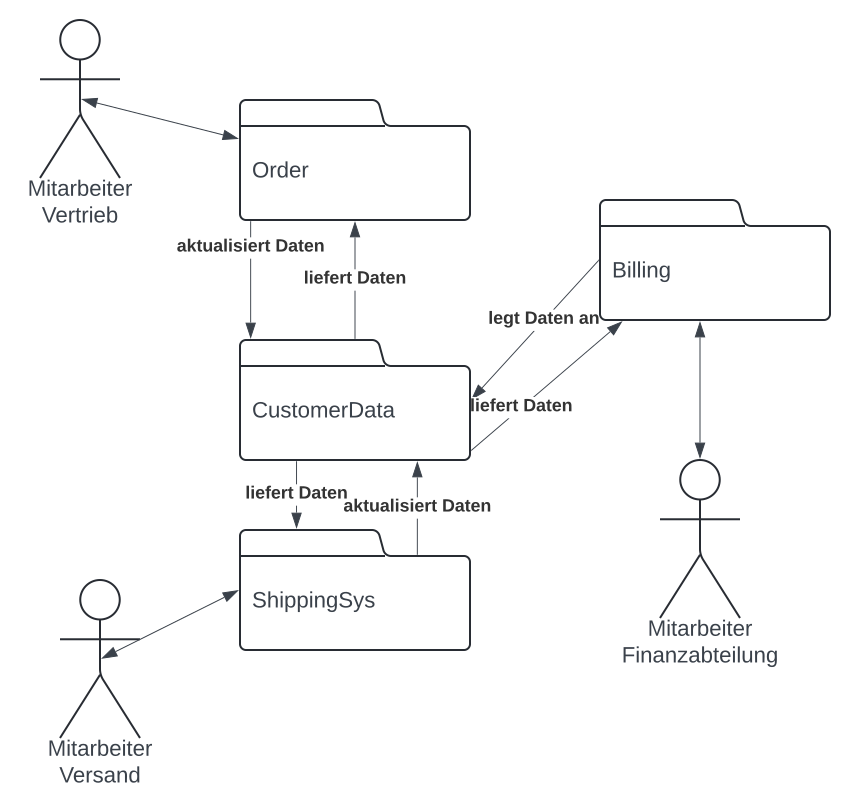
\includegraphics[scale=0.4]{chapters/Anhang/CheatSheets/img/contextdiagram}
    \caption{Beispiel für ein Kontextdiagramm. (Quelle: eigene)}
    \label{fig:contextdiagram}
\end{figure}
